\documentclass[10pt,twocolumn,letterpaper]{article}

\usepackage{cvpr}
\usepackage{times}
\usepackage{epsfig}
\usepackage{graphicx}
\usepackage{amsmath}
\usepackage{amssymb}
\usepackage{svg}

\usepackage{mathrsfs}

\usepackage{cite}
\graphicspath{ {images/} }
% Include other packages here, before hyperref.

% If you comment hyperref and then uncomment it, you should delete
% egpaper.aux before re-running latex.  (Or just hit 'q' on the first latex
% run, let it finish, and you should be clear).
\usepackage[breaklinks=true,bookmarks=false]{hyperref}

\cvprfinalcopy % *** Uncomment this line for the final submission

\def\cvprPaperID{****} % *** Enter the CVPR Paper ID here
\def\httilde{\mbox{\tt\raisebox{-.5ex}{\symbol{126}}}}

% Pages are numbered in submission mode, and unnumbered in camera-ready
%\ifcvprfinal\pagestyle{empty}\fi
\setcounter{page}{1}
\begin{document}

%%%%%%%%% TITLE
\title{\LaTeX\ Author Guidelines for CVPR Proceedings}

\author{First Author\\
Institution1\\
Institution1 address\\
{\tt\small firstauthor@i1.org}
% For a paper whose authors are all at the same institution,
% omit the following lines up until the closing ``}''.
% Additional authors and addresses can be added with ``\and'',
% just like the second author.
% To save space, use either the email address or home page, not both
\and
Second Author\\
Institution2\\
First line of institution2 address\\
{\tt\small secondauthor@i2.org}
}

\maketitle
%\thispagestyle{empty}

%%%%%%%%% ABSTRACT
\begin{abstract}
   The ABSTRACT is to be in fully-justified italicized text, at the top
   of the left-hand column, below the author and affiliation
   information. Use the word ``Abstract'' as the title, in 12-point
   Times, boldface type, centered relative to the column, initially
   capitalized. The abstract is to be in 10-point, single-spaced type.
   Leave two blank lines after the Abstract, then begin the main text.
   Look at previous CVPR abstracts to get a feel for style and length.
\end{abstract}

%%%%%%%%% BODY TEXT
\section{Introduction}

Please follow the steps outlined below when submitting your manuscript to
the IEEE Computer Society Press.  This style guide now has several
important modifications (for example, you are no longer warned against the
use of sticky tape to attach your artwork to the paper), so all authors
should read this new version.

%-------------------------------------------------------------------------
\section{Current methods}

In recent years, the field of Natural Language Generation (NLG) has expanded its repertoire
of solutions for text generation to include a variety of methods.
Models such as RNN's, Bi-LSTM, Transformers-based models (e.g.\ GPT), GAN's, among others, have evolved
to produce elaborate pieces of text for different specifics tasks.
Each method proposes a different approach to the task at hand.

\subsection{RNN}

Recurrent Neural Networks (RNN) are commonly used in sequence-to-sequence (seq2seq) tasks, such as text generation.
Simple RNN's have been adapted to overcome its own limitations, e.g.\ vanishing or exploding gradients,
introducing concepts such as Long Short Term Memory networks (LSTM) or even bidirectional LSTM's (Bi-LSTM).
LSTM's and Bi-LSTM have been used in many cases for text generation \cite{Bengali} \cite{lstm1} \cite{lstm2} \cite{lstm3}.
These models are still used in recent years.
Some studies \cite{embedds} use external word embeddings for the training process which can be seen as pre-trained
models for text generation.

In this work, we train a simple RNN with an Embedding layer, one LSTM module and a dense output layer.
The task of the RNN is to predict the next word for the text generation.
For this net, several hyperparameters can be set such as the number of LSTM layers, whether those layers
are bidirectional, pre-trained word embeddings, among many others.
The configuration that best minimized the cross-entropy loss was an embedding layer with no pre-trained embeddings,
three bidirectional LSTM layers and one dense output layer.
With this configuration, 1000 sentences were generated for comparison with alternative methods.

\subsection{Transformers}

With the introduction of \cite{attention}, new models for text generations task have arisen.
\cite{attention} introduces an Encoder-Decoder based architecture for machine translation tasks.
This architecture was ingeniously modified by \cite{bert} and \cite{gpt} to yield models such as BERT and GPT.
Both Generative Pre-trained Transformer (GPT) and Bidirectional Encoder Representations from Transformers (BERT)
are based on the idea of transformers and can be finetuned and
adapted for a variety of tasks \cite{gptapps1} \cite{gptapps2} \cite{gptapps3} \cite{gptapps4} \cite{gptapps5}.
These models have slowly replaced the RNN approaches.
As \cite{modernMethods} states: "Transformers disrupted sequence-based deep learning significantly.
The two variants of transformer models that we showed, BERT and GPT-2, outperform
previous approaches with RNNs".

GPT is widely known as a powerful tool for text generation.
Conversely, the BERT model alone has not been accepted as a strong generative model.
Some authors \cite{wang2019bert} have proposed workarounds to BERT limitations for text generation.

%------------------------------------------------------------------------
\begin{figure*}[t]
   \centering
   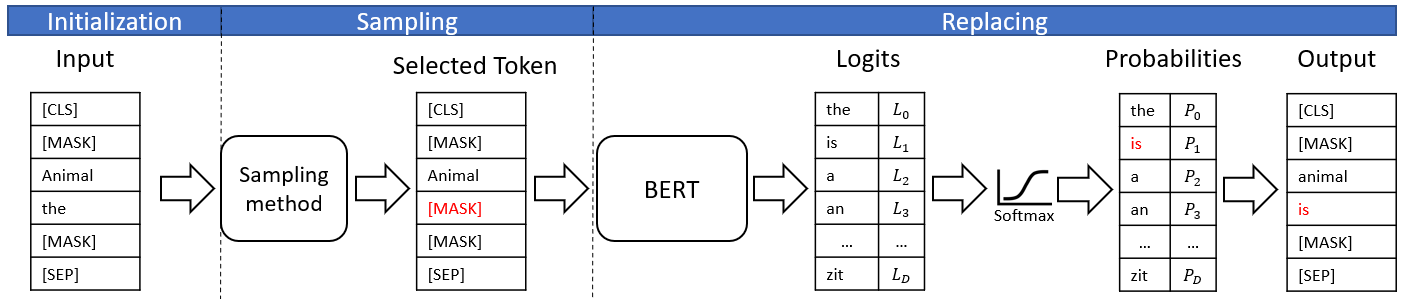
\includegraphics[scale=0.6]{BERTfunc.PNG}
   \caption{Process to use BERT as a generator.}
   \label{fig:BertFig}
\end{figure*}

\section{BertTextGenerator}
BERT is a language representation model designed to achieve state-of-art results
in several natural language processing tasks such as question answering and language inference.
BERT is trained on masked language modeling objective, in which it predicts a word given its
left and right context.
Given this behavior, it is possible to deduct that BERT is not the most
indicated model for text generation tasks.
However, \cite{wang2019bert} have demonstrated why it is possible to use BERT as a traditional
language model by means of showing that BERT is a combination of a 'Markov random field
language model (MRF-LM), with pseudo Log-Likelihood training'.
This conclusion allows using BERT as a generative model of sentences to either score a sentence or
sample a sentence.

To generate text with BERT the process is composed by 3 main steps described as follows and illustrated in the Figure \ref{fig:BertFig}:

\begin{itemize}
\item Initialization: It is necessary to initialize the sequence with a random initial state, this can be either an all-mask sequence,
i.e.([MASK], ...,[MASK]), an all-random sequence, or a combination of these, i.e. (50\% [MASK] tokens and 50\% random tokens).
\item Sampling: At each iteration, it is necessary to choose which token of the sequence will be masked, in \cite{wang2019bert}
they propose three different methods to carry out the sampling, these methods are described as follows:
\begin{itemize}
   \item Sequential: The sequence is masked from left to right one token at a time at each iteration.
   \item Parallel sequential: The sequence is masked choosing at random one token at each iteration.
\end{itemize}
\item Replacement: Finally, the sequence with the masked token is passed to BERT to produce a tensor of logits $L$ of
the length of its vocabulary $v (v \approx 30K)$. The logits are interpreted as a probability distribution of how related
are each one of the tokens in the BERT vocabulary with the current sequence. Finally, the logits are normalized using a
softmax function to retrieve the probability of each token to be inserted on the sequence and based on this probability
the new token is selected.
\end{itemize}

The initialization is made only once at the beginning of the generation process, the sampling and the replacing are
made once for each iteration of the model.

%------------------------------------------------------------------------
\subsection{Attention mechanism}
The attention mechanism is composed by a feed forward neural network that is trained to
identify the more relevant components in the context in order to predict a new token.

For example, take the sentence "the animal didn't cross the street because it was too tired",
as a human it is easy to know that in the sentence the pronoun "it" refers to the subject "the animal"
and the verb "was" is the correct conjugation of the verb "To be" for the third person, but for an
algorithm is not easy to know these relationships and that is the task of the attention mechanism.

For example, In the sentence "the animal didn't cross the street because it was too tired"
some attention heads would focus on the verb "was", other attention heads would focus
on the special tokens "[CLS]" and "[SEP]" that represent the beginning and the end of the sentence
respectively, finally other attention heads would focus on the word "animal". In this way BERT can
understand which parts of the context are more relevant.

\begin{figure}
   \centering
   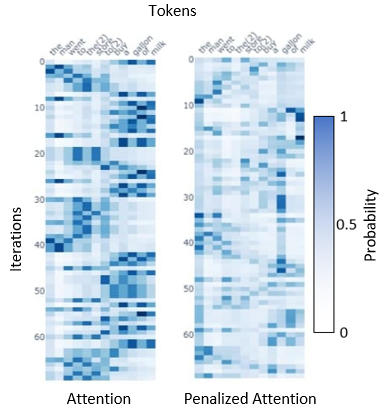
\includegraphics[scale=0.7]{attComp.PNG}
   \caption{Comparison of the behavior of the proposed sampling methods.}
   \label{fig:AttentComp}
\end{figure}

\subsubsection{Using the attention mechanism to improve the sampling method.}
When a token is predicted, it is possible to know which tokens of the context were more relevant to
retrieve the prediction based on the attention weights.
This information is a very meaningful insight to improve
the way in which the sampling method is made.

We propose a new sampling method based on the attention
weights returned by BERT when a prediction is done.

\paragraph{Attention based sampling}
First, we design a sampling method totally based on the attention weights,
when a token was replaced in the past iteration we retrieve and summarize the
attention information corresponded to the replaced token by means of averages
inside and between the encoders to get a unique measure of the attention, then
we normalize the result to get a probabilistic interpretation and make the new
sample based on this probability, in this way we wanted to sample the more related
tokens to the one that was replaced to check if this tokens preserve his meaning in the sequence.

However, we found that the attention mechanism creates very strong correlations between
few tokens of the sequence, then the sample got stuck always choosing the same tokens among
all the iterations.
To solve this behavior, we add a penalization to those tokens that were
chosen several times, in the next section we describe the new method.

\paragraph{Penalized attention sampling}
This method is very similar to the previous one, however, we include a penalization factor
to those tokens that were chosen several times, in that way the sampling method makes a better
exploration of the sequence based on the attention information and as a result we get better
generations.

below we describe the procedure to develop the sampling method in the iteration $t$:

\begin{itemize}
\item Step 1: Retrieve the attention masks of the iteration $t-1$ ($a$), then get the average value of the attention masks $A_{p,e}$ for each position $p$ inside each one of the encoders $e$.
\item Step 2: Get the average value of the attention mask $totalA_{p}$ for each position over all the encoders.
\item Step 3: For each position $p$, there is a counter $c$ that register how many times the position $p$ has been selected to be replaced.
\item Step 4: The average value of the attention masks $totalA_{p}$ is divided by the counter $c$ to create a penalization.
\item Step 5: Normalize the result of the step 4 to get a probability distribution $P$.
\item Step 6: Sample randomly with distribution $P$ the new token to be replaced.
\end{itemize}

In the step 1 we summarize the information of the attention inside each one of the encoders,
then in the step 2 we combine the information of the different encoders to obtain a single
measure of the attention, the step 4 is useful to help the method to avoid that the sampling
method get stuck sampling always the same positions given its strong relation with the current
context, finally the steps 5 and 6 creates a probability distribution based on the penalized attention
and sample the new token to be replaced.

Finally, in the Figure \ref{fig:AttentComp} it is possible to see how the probability of choose a token evolves
during the iterations for each one of the tokens, it is possible to note how the attention method
get stuck during several iterations in the same areas of the sequence, for example, during the iterations
10 to 16, the probability was focus on the last 4 tokens of the sequence.
While in the penalized attention is possible to see a more balance probability distribution inside each iteration
and the sampling method is not focus in only few parts of the sequence.
%------------------------------------------------------------------------
\subsection{Finetuning}
BERT is a powerful model pre-trained on a broad set of text composed by the whole
Wikipedia and Brown corpora.
One of its main feature is its adaptability to a plethora of different tasks,
by means of a fine-tuning on specific domain set.
Typical fine-tuning techniques depend on the final task that the user requires BERT to perform.
For example, considering classification tasks such as sentiment prediction and text classification,
the fine-tuning will be focused on the [CLS] token, a special token used in the pre-training phase for the task
of \textit{next-sentence-prediction} and specifically designed for classification applications.

Text generation is not a usual task for BERT.
In this case, the fine-tuning aims to make the model understand the structure of the text,
in order to mimic it at inference time.
We have implemented a fine-tuning procedure that relies on a \textit{Cloze} task, similar to the one adopted in the
 original training \cite{wang2019bert}.
This consists on replacing a percentage (15\% by default) of the tokens for each sentence with a [MASK] token and let
BERT predict the blanks. The logits outputted by the model are then used to compute the cross-entropy
loss with respect to the original token that were replaced.

This method allows the final user to start from a pretrained model and fine-tune it on a specific
text corpus in order then to make it generate text similar to the original one.
This approach also works  in the case that a pretrained model is not available in th language selected by the user.
In this case, the user can simply start from a cross-language model [...]

\subsubsection{Structure of the text}
The default vocabulary of the tokenizer contains around 1000 unused tokens, whose weights are randomly initialized.
Typically, these tokens are replaced with domain specific words, so that during the fine-tuning phase
the model will be able to learn their representation.
We have extended this idea in order to comprehend also tokens that define the structure of the text like
'\textbackslash n' and '\textbackslash t'.
Note that, simply adding these tokens to the vocabulary would have no effect.
These tokens in fact, are typically replaced even before the tokenization, during the normalization step of the Tokenizer pipeline [].
However, these tokens can be really important, especially in the task of text generation.

To solve this problem we have implemented a Formatter class that helps the user to format the text in order
to preserve the important tokens.
The Formatter replaces a user specified set of tokens that need to be preserved, with some unused-tokens.
The replacement happens before the tokenization, in this manner, during the fine-tuning the model will be able to learn
the position of these important tokens.
The unused tokens are then replaced back with the original ones after the generation.

Using this method we were able to fine-tune a model able to learn the famous tercet structure of Dante's Divine Comedy \ref{}.

\subsubsection{Sentiment generation}
\label{sentiment}
An important aspect of BERT tokenizer are special tokens like [CLS], [MASK] and [SEP].
As the name suggests, these are tokens with special functions.
The tokenizer gave the possibility to define new special tokens.
We have taken advantage of this opportunity to define a new method to generate text with a specific sentiment or label.

Consider a domain set $\mathcal S$ of sentences each one with an attached label $y\in \mathcal Y$, i.e.\ a text whose label-set are the two possible sentiments $\mathcal Y =\{pos, neg\}$.
The method consists of three main steps:

\begin{itemize}
\item For each sentiment in the label set $y\in\mathcal Y$, we define $n$ (3 by default) special tokens $[y_i]\;\; for\;\;i=1,\ldots n$.
In the case of $y=pos$ for example the set of special tokens will be $\{\text{[pos-1]}, \text{[pos-2]}, \text{[pos-3]}\}$
\item Before the fine-tuning each sentence $s\in\mathcal S$ is tokenized, and the special tokens corresponding to its label are appended at the beginning of the list of tokens.
\item The fine-tuning is performed. During this step the model will build a relation among the special tokens of a sentiment and the specific words
related to it.
\end{itemize}
To generate the text with a given sentiment, the special tokens related to that sentiment are used as a seed to create
a context on top of which BERT can start to generate.
$$\begin{bmatrix}\text{[CLS]} \end*{}
   \begin*{}&\underbrace{ \;\; \text{[pos-1]} \;\; \text{[pos-2]} \;\; \text{[pos-3]}}_{seed}&\end*{}
   \begin*{}
      \text{[MASK]} &\text{[MASK]}&\ldots
   \end{bmatrix}$$

This method, even in its simplicity, showed its efficacy in generating positive and negative italian tweets about football.
In addition, this method will allow the possibility to consider even more than two labels.
%------------------------------------------------------------------------
\begin{table}
\centering
\begin{tabular}{lllll}
\hline
\multicolumn{1}{c}{}                            & \multicolumn{4}{c}{\vcell{Model}}                  \\[-\rowheight]
\cline{2-5}
\multicolumn{1}{c}{\multirow{}{}{Parameter}}                           & \begin{tabular}[c]{@{}l@{}}Parallel\\ 1\end{tabular} & \begin{tabular}[c]{@{}l@{}}Parallel\\ 0.15\end{tabular} & Sequential & Attention  \\
\hline
Avg\_len                                       & 40        & 40           & 40         & 40         \\
Std\_len                                       & 5         & 0            & 5          & 0          \\
Masked\_p                                      & 1         & 0.15         & 1          & 1          \\
Sample                                         & True      & True         & True       & True       \\
Init\_mask\_p                                  & 1         & 1            & 0          & 1          \\
Temperature                                    & 1         & 1            & 1          & 1          \\
Top\_k                                         & 0         & 100          & 100        & 100        \\
\hline
\end{tabular}
\caption{Parameters configuration of the best models obtained for each generation method.}
\label{tab:parameters}
\end{table}



\begin{table}[]
\begin{tabular}{lllll}
\hline
\multicolumn{1}{c}{} & \multicolumn{2}{c}{Bleu} & \multicolumn{1}{c}{\multirow{}{}{}} & \multicolumn{1}{c}{} \\ \cline{2-3}
\multicolumn{1}{c}{\multirow{}{}{Model}}   & WT103       & TBC        & \multicolumn{1}{c}{\multirow{}{}{Perplexity}} & Self-Bleu  \\ \hline
Original \cite{wang2019bert}                & 7.06        & 7.8        & 279.1        & 10.06                                            \\
Original*                            & 6.86        & 7.14        & 270.6             & 8.43                                  \\
Parallel-1                                 & 6.62        & 7.21       & 287.6                    & 6.83                           \\
Attention                                 & 8.15        & 6.59       & 386.6                  &  11.88                          \\
Parallel-0.15                              & 8.79            & 7.11           & 1241         & 12.02                                       \\
Sequential                                & 5.73            & 7.27           & 374.2          & 7.05                                      \\
RNN (WT)                                & 8.54            & 2.9           & -                  & 15.23                              \\
RNN (TBC)                                & 5.73            & 7.27           & -                & 7.45                                \\ \hline
\end{tabular}
\caption{Quality and diversity metrics of model generations.}
\label{tab:results}
\end{table}

\section{Experiments and evaluation}

The evaluation of generated text is not a simple task.
Some evaluations rely on intrinsic or extrinsic techniques.
Within these techniques metrics such as n-gram overlap metrics (f-score, bleu, self-bleu, rouge, meteor),
distance-based metrics, diversity metrics, content overlap metrics or even grammatical feature based
are taken into account.
Each metric reflects different results.
For example, the self-bleu represents the diversity of the text \cite{texygen}.
But this metrics are not perfect and can also be deceived.
\cite{evaltextgen1} explains the different struggles these measures have.
For example, it states that "a language model optimized only for perplexity
may generate coherent but bland responses."
In this sense, it is not simple to evaluate a text generator model based on a single metric.

% Grid search explanation
% Best model 1000 sents
% Corpus Bleu, perplexity and rouge
% Self-Bleu and n-Grams

We have made a Grid Search to analyze the behavior of the generations with the variation of the parameters,
and to choose the best combination of parameters for each one of the sampling methods. For each one of the
combinations of parameters we have made five different generations each one with 500 text lines generated,
then we calculated different measures to analyze the quality and the diversity of the generations like
Corpus-Bleu on Wikitex-103 and TBC, rough and \%Unique-Ngrams. We select the three bests models for each
generation method by means of comparing all the measures. Finally, we generated 1000 text lines with each one
of the models, we evaluate the final generations and based on the results we choose the best combination of
parameters for each model, in table \ref{tab:parameters} we report the parameters of each model.

In table \ref{tab:parameters}, we report the Bleu scores with respect to WT103 and TBC for the best models we found,
the results of the original paper \cite{wang2019bert}, the results of the original paper but evaluating the generated
text with the Texygen library, and a RNN we trained on WT103.5 and TBC, in the following section we discuss more about
the RNN model. It is possible to note that the proposed attention method is very near of the base line marked by the
original paper, even outperforming the base line in the corpus-Bleu measure with respect to WT103.

\subsection{Convergence of the attention sampling method}
We have compared also the converge of the attention method with respect to the original sampling method (parallel).
To do this we have run 80 generation experiments. Each sentence was initialized with a list of 25 [MASK] tokens and
generation was runnign for 150 iterations. During each iteration we measured some statistics like the number of the
iterations needed to replace all the original [MASK] tokens. This is an indicator of the speed at which the method is able to create
a context for the sentence. Considering the original parallel method and the vanilla attention, in average more than 80
iterations were required over 150. This means that the model had less than half the iterations to try to replace tokens
with a complete sentence. Moreover the results showed a very high variability.
On the other hand the attention method penalized showed a much faster replacement of the initial [MASK] tokens.
\begin{figure}[t!]
   \centering
   \includesvg{test.svg}
%   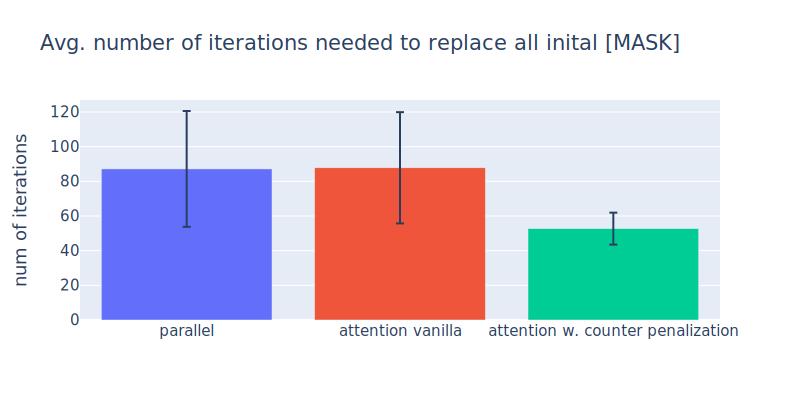
\includegraphics[scale=0.3]{test.svg}
   \caption{
   }
   \label{fig:ReplaceMask}
\end{figure}

This behavior reflects on a faster convergence of this method. We can see also in \ref{fig:Recall}

\begin{figure}[t!]
   \centering
   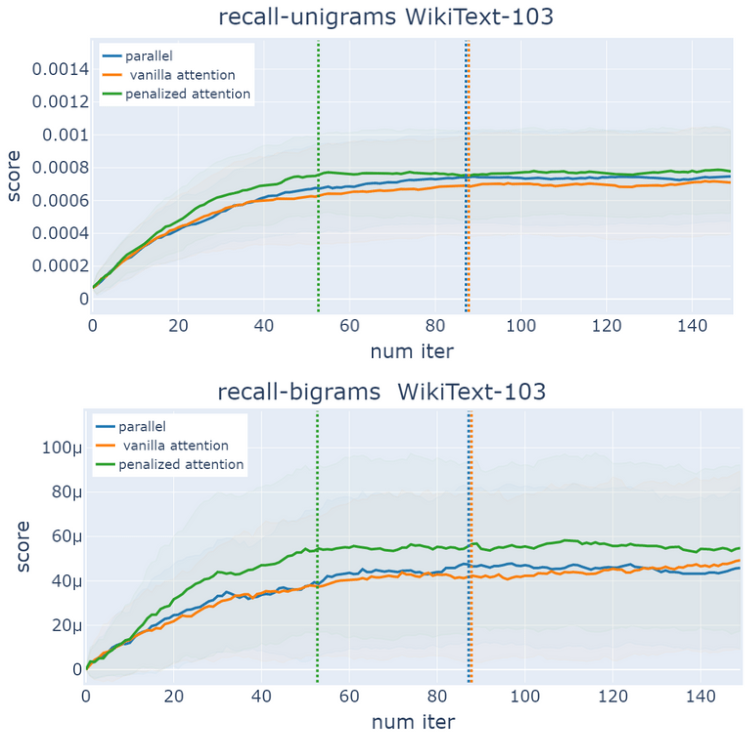
\includegraphics[scale=0.4]{recall.png}
   \caption{Average recall score of unigrams and bigrams w.r.t WikiText-103
   at each iteration. The dashed lines correspond to the avg num of iterations needed
   to replace the initial mask tokens}
   \label{fig:Recall}
\end{figure}

\subsection{Italian generation: finetuning experiments}
In order to test the goodness of the fine-tuning implementation we have performed three experiments. []
All the experiments have been performed on Italian sets of text and for all the experiments we started from a
pretrained italian BERT model
%, freely downloadable from huggingface [].

\paragraph{Motivational quotes} The first experiment aimed at showing the functionality of the fine-tuning method.
To do that we have gathered a small set of motivational quotes.
The set was constructed scraping from different sources, and the quotes were preprocessed in order to make them
all structured in the same way:
\begin{quote}
   A motivational quote - (anonymous)
\end{quote}

The results were quite surprising, the model was able to learn the structure of the quote (quote-dash-parentheses-author)
and to generate some meaningful text. These are some example of the quotes generated:

\begin{quote}
   se vuoi davvero fare una cosa, e meglio se la smetti di farla. ( thomas edison )
\end{quote}
\begin{quote}
non hai nulla da fare, tutti i giorni, se non stai cercando di fare tutto cio che e necessario. ( norman bates )
\end{quote}
\begin{quote}
   quando muori, la vita finisce. non ci resta che aspettare finche non muori, perche non sai cosa ti aspetta ( anonimo )
\end{quote}

Obviously not all the quotes were this good. A lot of generation were stucked on repetitions of the same words or tokens.
This is a common problem that we have found on all the generations with BERT that we have done.
The sampling methods that outputted the most reliable quotes seemed to be the attention and the sequential.

\paragraph{Dante's divine comedy} The second experiment was focused on the structure of the text,
for this part we have used Dante's Divine Comedy. The model was fine-tuned on tercets (groups of three lines) instead of single lines.
\begin{quote}
   Nel mezzo del cammin di nostra vita\\
   mi ritrovai per una selva oscura,\\
   ché la diritta via era smarrita.\\
\end{quote}
Each tercet was preprocessed replacing '\textbackslash n' with 'unused1' tokens as explained in \ref{}.

%\begin{quote}
%['Nel', 'mezzo', 'del', 'cammin', 'di', 'nostra', 'vita', \textbf{'unused1'},
% 'mi',
% 'ritrovai',
% 'per', \ldots
%% 'una',
%% 'selva',
%% 'oscura,',
%% \textbf{'unused1'},
%% 'ché',
%% 'la',
%% 'diritta',
%% 'via',
%% 'era',
%% 'smarrita.',
%% \textbf{'unused1'}]
%\end{quote}

\begin{quote}
 che mai non m ’ io coglia ;\\
 e non abbracci che li si ridesse,\\
 che piu tempo fece prodente.\\


 ma vidi io di lo vento che\\
 del son s ’ accesi io :\\
 per tanto piacer che questo venisse il triscio ».\\


 ma gia di queste le zanne\\
 sonn piu, si malicce,\\
 che prima l ’ occhio non era in ciel ;\\

\end{quote}

%\begin{quote}
%
%e disse a me : ‘ e tu? ’\\
%piu in la che vidi, piu non si facea ;\\
%questo e ’ l padre mio, che e con me ».\\
%
%e cato e cato, e in lui\\
%si fece ’ l uno e un altro,\\
%si che ’ l le membra e lo spirito movea ».\\
%
%sappi pero che la tua mente e buona,\\
%che si fa la volonta di dio,\\
%com ’ e stata fatta l ’ arte del mondo,\\
%che non e morta.\\
%
%“ e ’ l viso mio “ chinato ”,\\
%e ’ l vidi correr dietro a me\\
%si tentenno e disse : « loco, loco! ».\\
%\end{quote}

All the '\textbackslash n' tokens present in the quote were automatically generated by the model.
Also in this case the attention sampling method seemed the one able to reproduce the structure in the best way.


\paragraph{Sentiment generation} In this case we have used a dataset [] composed by num italian tweets.
Each tweet has associated a sentiment score for each one of 4 possible labels
$\mathcal Y = \{\text{POSITIVE}, \text{NEGATIVE}, \text{MIXED}, \text{NEUTRAL}\}$ and a sentiment label corresponding
to the sentiment with the highest score.
The dataset was highly imbalanced, with respect to the last two classes, so we have considered only the first two.
The dataset was preprocessed as explained in \ref{sentiment}; in addition a set of tokens was added to the vocabulary
in order to deal with '@tags' and '#hashtags'.\\

[POSITIVE]:
\begin{quote}
   ronaldo tante complimenti per per il tuo bellissimo debutto, dopo aver visto il tuo punto forza e auguri @\_/juventusfc #juventusfc #juventusfc?
\end{quote}

[NEGATIVE]:
\begin{quote}
   ronaldo??? molto bene? molto bene??? non si vince mai con sportivita e fiducia non ti preoccupare hai dimostrato di non poter faticare a nulla
\end{quote}


%-------------------------------------------------------------------------
\section{Conclusions}
In this project we explored the usage of BERT as a text generator,
focusing in particular on the sampling methods.
Our new attention method was able to reach the results obtained in the original paper
improving the convergence time, and the number of iterations needed.

Anyway as in the original paper, the results of BLEU score on the generation of a wide body of text
showed the unreliability of BERT in text generation, due to incapacity of controlling the generation.
In particular, a typical problem that we have encountered during the generation was that in
a considerable number of iterations the model was stuck in a bad part of the
configuration space i.e. all '.' tokens or repetition of groups of tokens.
The consequence was that BERT was keeping replacing the tokens with the same ones until the last iteration.

Nonetheless, our experiments showed the possibility to still apply the model
on specific domains i.e quotes, through a fine-tuning.
In this case, BERT were able to clearly understand
the structure and generate some meaningful text.

Due to high variability of the results, we can conclude that no sampling method was clearly
outperforming the others. This suggests the possibility of future exploration in other parts
of the generation method. In particular it could be interesting a further investigation
of the resampling part and the implementation of a scheduling of the temperature of the logits,
in order to help the generation method to not get stuck in the early stages of the generation.

\bibliographystyle{ieeetr}
\bibliography{egbib}

\end{document}
